% !TeX spellcheck = fr
% !TeX encoding = UTF-8
\documentclass{beamer}

\usepackage{fontspec}
\usepackage{xltxtra}

%\usetheme{Boadilla}
\usetheme{PaloAlto}
%\usetheme{Berlin}
%\usecolor{}

%\usepackage{minted}


%\setmainfont{Linux Libertine O}
\usepackage[english,french]{babel}

\usepackage{hyperref}
\usepackage{graphicx}

\institute{Univ. de Neuchâtel}

\title{Exploiter les données}
\subtitle{Introduction à la textométrie avec \textsc{txm}}
\author{Jean-Baptiste Camps \& Simon Gabay}
\date[FoPhil -- 14 févr. 2018]{Formation en philologie numérique:\\ encoder, exploiter, diffuser\\
12-16 février 2018}

\makeatletter 
         
        \AtBeginSection[]{% 
        \begin{frame}{Plan}%
        \small
        \tableofcontents[currentsection]%
        \end{frame} }

        %\AtBeginSubsection[]{% 
	%\begin{frame}{Plan}%
	%\small
	%\tableofcontents[currentsection,currentsubsection]%
%\end{frame} }


\makeatother 
    
    
\begin{document}

\maketitle
%\frontmatter 
  

\begin{frame}{De la production des données à l'exploitation}
	
	\begin{columns}[T]
		
		\begin{column}{0.62\textwidth}
			
			\textsc{Ceux-ci collectent les données}
			
			\centering
			
			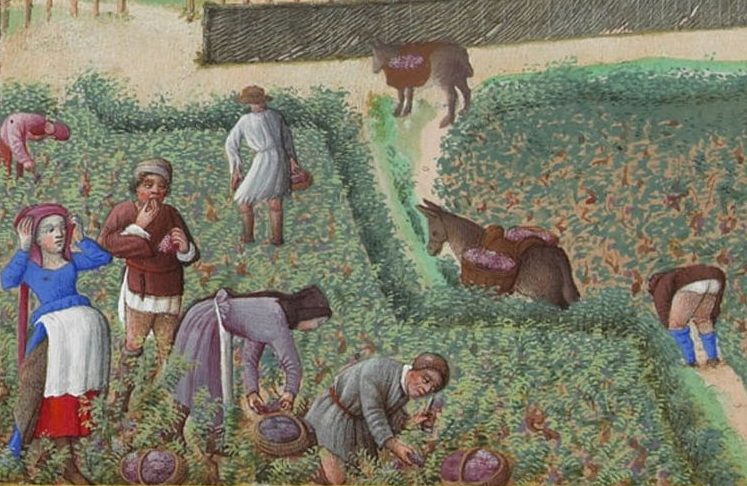
\includegraphics[width=\textwidth]{img/vendange.jpg}
			
		\end{column}
			\begin{column}{0.38\textwidth}
		
		\textsc{Ceux-là les exploitent}
		
		\centering
		
		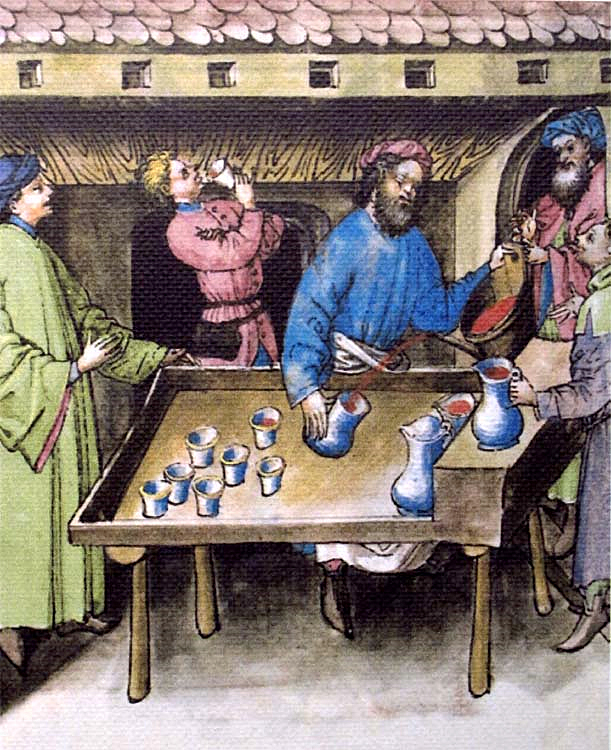
\includegraphics[width=\textwidth]{img/vin2.jpg}
		
	\end{column}
		
	\end{columns}
	
\end{frame}

%\mainmatter 

\begin{frame}{Objectifs}
	
	\begin{itemize}
		\item S'initier à la \alert{textométrie},
		\begin{itemize}
			\item créer des corpus;
			\item les interroger;
			\item faire (un peu) d'analyse quantitative.
		\end{itemize}
		\item dans le cadre d'un logiciel ``tout en un'' et convivial, 
	\alert{\textsc{txm}} \cite{Heiden2010},
		\item sur des cas tirés de la littérature du XVII\ieme{} siècle.
	\end{itemize}


\begin{block}{La textométrie selon \cite{Pincemin2008}}
	\begin{quote}
		La   textométrie développe  les  possibilités  de  consultation  et  d'analyse  de
		corpus  textuels  en  faisant  appel  à  des  décomptes  et des
		modélisations  statistiques  et  en  combinant  aux  possibilités
		de repérage d'occurrences des calculs de tri, de sélection et
		de réorganisation statistique.
	\end{quote}
\end{block}
	
\end{frame}


\begin{frame}[fragile]
\frametitle{\textsc{txm}: un logiciel de textométrie}


\begin{columns}
	\begin{column}{0.30\textwidth}
	\begin{center}
	
\includegraphics[width= 0.8\textwidth]{img/txm.png}
	\end{center}

\url{http://textometrie.ens-lyon.fr/}

\textit{Base de français médiéval:} \url{http://txm.bfm-corpus.org/}.
	\end{column}
	\begin{column}{0.66\textwidth}
		\begin{itemize}
			\item Logiciel libre et multiplateforme;
			\item développé à l'ÉNS-LSH de Lyon;
			\item dévoué à la textométrie;
			\item repose sur des technologies de référence:
				\begin{itemize}
					\item \textsc{xml/tei} pour les données;
					\item \textsc{r} pour l'analyse statistique;
					\item \textsc{cqp} pour l'interrogation de corpus;
					\item \texttt{TreeTagger} pour l'annotation.
				\end{itemize}
		\end{itemize}
	\end{column}
\end{columns}
\end{frame}


\begin{frame} 
  \frametitle{Plan} 
  \tableofcontents
\end{frame}

\section{Mise en jambe: \textit{Andromaque}}

\begin{frame}{Création d'un corpus à partir de notre édition d'\textit{Andromaque}}

\begin{enumerate}
	\item Fichier, importer, import XML/W + CSV;
	\item sélectionner le dossier avec les sources et remplir les paramètres du corpus;
	\item lancer la création du corpus.
\end{enumerate}

\end{frame}

\begin{frame}{Premières fonctionnalités}
\begin{enumerate}
\item Consulter la description du corpus;
\item parcourir l'édition;
\item regarder le lexique;
\item ouvrir l'index, y chercher les occurrences de 'Seigneur';
	\begin{enumerate}
		\item clic-droit, envoyer vers les concordances;
			\begin{enumerate}
				\item double-clic sur une occurrence pour aller au texte;
			\end{enumerate}
		\item clic-droit, envoyer vers les cooccurrents;
			\begin{enumerate}
				\item aller d'un cooccurrent aux concordances, puis au texte
			\end{enumerate}
		\item clic-droit, envoyer vers la progression;
	\end{enumerate}
\end{enumerate}

\end{frame}

\begin{frame}{Partitions et quelques éléments descriptifs}
\begin{enumerate}
\item créer une partition, en sélectionnant la structure \texttt{sp} et l'attribut \texttt{\@who};
\item consulter les dimensions;
\item créer une table lexicale, expérimenter avec les tris, la fusion ou suppression des colonnes, etc.
\end{enumerate}
\end{frame}

\begin{frame}{Statistiques de base}
À partir de la table lexicale créée,
\begin{enumerate}
\item calculer les spécificités;
\item quels sont les mots les plus spécifiques d'Oreste? de Pylade?
\item en sélectionner quelques uns qui sont pertinents;
\item calculer le diagramme en bâton des lignes sélectionnées.
\end{enumerate}
\end{frame}

\begin{frame}{Qu'en déduire?}
	
	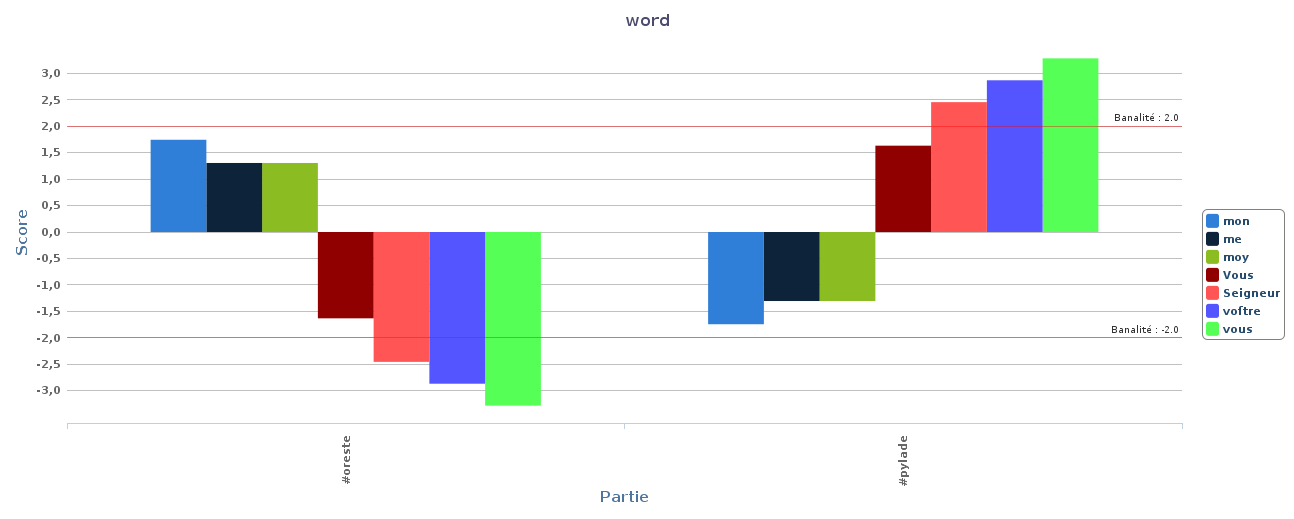
\includegraphics[width=\textwidth]{img/graphique_word_Oreste.png}
	
\end{frame}

%TODO: ajouter formule et expliquer maths des spécificités, si temps.


\frame{Prêts à passer aux choses sérieuses?}

\section{Importer des données et créer un corpus}

\begin{frame}{Différents modes d'import}
	
	\begin{description}
		\item[flemmards] import (avec ou sans métadonnées complémentaires)
		depuis 
		\begin{itemize}
			\item presse-papier;
			\item des fichiers \texttt{txt} ;
			\item traitement de texte.
		\end{itemize}
		\item[XML] XML/ TEI ou autre;
		\item[spécifiques] formats de logiciels de textométrie.
	\end{description}
	
\end{frame}

% Le corpus

\begin{frame}[fragile]
\frametitle{Corpus du jour: un peu de théâtre du XVII\ieme{} siècle}

Corpus constitué pour le cours d'aujourd'hui:

\begin{itemize}
	\item source: Paul Fièvre,  \url{http://www.theatre-classique.fr/};
	\item documents encodés en \textsc{xml}/\textsc{tei} (ou dans plusieurs \textsc{xml/tei});
	\item corpus de \alert{36} pièces de théâtre en vers du XVII\ieme{} siècle,
	\item appartenant à trois genres principaux:
		\begin{itemize}
			\item comédie,
			\item tragédie,
			\item tragi-comédie.
		\end{itemize}
	\item sélectionnées un peu au hasard,
	\begin{itemize}
		\item mais en essayant de conserver un équilibre entre les genres principaux (comédie, tragédie, tragi-comédie),
		\item d'avoir des pièces de longueur similaire (entre 1250 et 2000 vers),
		\item un équilibre entre les auteurs (4 pièces par auteur),
		\item et entre les générations (4 auteurs par génération).
	\end{itemize}
\end{itemize}

\end{frame}

\begin{frame}{9 auteurs, 2 générations}
	%	Auteurs, approximativement de deux générations un peu différentes du XVII\ieme{} siècle,
	\begin{columns}[T]
		\begin{column}{0.45\textwidth}
			G1, c.~1630-1650
			\begin{itemize}
			    \item Pierre Du Ryer \\(fl. 1628-1655);
			    \item Georges de Scudéry\\ (fl. 1631-1643).
				\item Jean de Rotrou\\ (fl. 1635-1649);
				\item Paul Scarron\\ (fl. 1648-1660);
			\end{itemize}
		\end{column}
		\begin{column}{0.45\textwidth}
			G2, c.~1650-1690
			\begin{itemize}
				\item Claude Boyer\\ (fl. 1646-1697);
				\item Thomas Corneille\\ (fl. 1651-1696)
				\item Molière\\ (fl. 1655-1673)
				\item Jean Racine\\ (fl. 1664-1691);
			\end{itemize}
		
		\end{column}
	\end{columns}
	
			Et un monstre sacré, \textbf{Pierre Corneille} (fl. 1629-1675).
	
\end{frame}

\begin{frame}{Sources et pré-traitements}
	
	
	 \begin{itemize}
	 	\item Graphies modernisées (dommage… mais va faire notre affaire dans ce cas précis);
	 	\item Faut-il supprimer la distinction majuscule/minuscule?
	 		\begin{itemize}
	 			\item Pour: suppression de biais éditoriaux.
	 			\item Contre: les majuscules peuvent conserver de l'information syntaxique.
	 		\end{itemize}
 		\item Veut-on garder tout ce qui est extérieur aux répliques (liste des personnages, page de titre, etc.)?
 			\begin{itemize}
 				\item Peut être retiré grâce à la structuration \textsc{xml/tei}.
 			\end{itemize}
	 	\item pas de lemmatisation: possibilité de lemmatiser et annoter automatiquement.
	 \end{itemize}
	
\end{frame}

\begin{frame}[fragile]
\frametitle{Transformations avant l'import}
	
	Dossier \texttt{xsl}, feuille \texttt{source\_to\_txt.xsl} (2.0), deux sorties:
	
	\begin{enumerate}
		\item fichier \texttt{metadata.csv}: métadonnées des documents extraites automatiquement des fichiers \textsc{tei} (\texttt{teiHeader} et page de titre, \texttt{docDate});
		\item dossier \texttt{txt}: transformation en \texttt{txt} des pièces:
			\begin{itemize}
				\item passage en bas de casse;
				\item suppression du \texttt{teiHeader};
				\item suppression du \texttt{castList} et des mentions de personnage, \texttt{speaker};
				\item suppression du \texttt{front}, des \texttt{docTitle}, \texttt{docDate}, \texttt{docAuthor}, \texttt{docImprint}, \texttt{printer}, \texttt{performance}, \verb|div[\@type='dedicace']|;
				\item suppression des titres, notes.
			\end{itemize}
	\end{enumerate}
	
\end{frame}

\begin{frame}{Import \texttt{txt} + \texttt{csv}}
	
	\begin{enumerate}
		\item sélectionner le répertoire de sources \texttt{txm\_import1\_txt} (contenant fichiers \texttt{txt} et métadonnées \texttt{csv},
		corpus tronqué pour gagner un peu de temps);
		\item paramétrer l'import (nommer le corpus THEATRENEUCHTXT);
		\item demander la lemmatisation;
		\item vérifier que les métadonnées sont bien comprises;
		\item lancer l'import;
		\item (regarder le log de l'import);
		\item une fois l'import réussi, jeter un œil à la description, à l'édition, etc.
	\end{enumerate}
	
\end{frame}

% Import XML amélioré, avec XSLT intermédiaire, lemmatisation, etc. etc.

\begin{frame}{Import \texttt{xml/w} + \texttt{csv} amélioré}

\begin{enumerate}
	\item sélectionner le répertoire de sources \texttt{txm\_import2\_xml} (contenant fichiers \texttt{xml} et métadonnées \texttt{csv},
complet);
	\item paramétrer l'import (nommer le corpus THEATRENEUCHXML);
	\item demander la lemmatisation;
	\item vérifier que les métadonnées sont bien comprises;
	\item \alert{associer l'\texttt{xsl} 2.0 de pré-traitement, \texttt{import\_xml\_filtre.xsl}};
	\item lancer l'import;
	\item (regarder le log de l'import);
	\item une fois l'import réussi, jeter un œil à la description, à l'édition, etc.
\end{enumerate}

\end{frame}


\section{Interroger les données}

%interrogation des mots

%interrogation des lemmes

%rudiments de CQL (CQP)

%Partitions par genre, auteur, texte. Table-lexicale, lemmes ou formes

\section{Quelques notions d'analyse quantitative}

\begin{frame}[fragile]
\frametitle{Approches principales: la forme (linguistique) ou le fond (sémantique)?}

Sans prétention à l'exhaustivité, on peut distinguer deux approches principales qui font emploi des méthodes que nous allons présenter:
\begin{itemize}
	\item \textbf{approche stylométrique}, qui se préoccupe d'attribution, datation, localisation des textes; pour ce type d'approche, on va s'intéresser à l'information graphique (variantes d'orthographe), flexionnelle (terminaisons verbales, …), etc. On va aussi tendre à s'intéresser seulement aux \alert{mots les plus fréquents} (mots-outils, mots-vides), les moins sensibles aux variations intentionnelles de leurs auteurs (genre, sujet, etc.). Le \textbf{sens des textes nous indiffère} (ou presque).
	\item \textbf{approche sémantique}, lexicométrique, etc., qui est à peu près l'inverse de la précédente: intérêt pour les mots en tant que lemmes et leurs rapports entre eux (cooccurrences), pour les réseaux de sens, les thèmes des textes, etc.
\end{itemize}
Très schématique, mais nous en reparlerons plus tard.
\end{frame}

% Quelques stats desc?

% Problématique: les genres littéraires (thématique)

% Problématique: les auteurs (stylométrie)



\appendix

\begin{frame}[fragile]
\frametitle{Bibliographie} 

\begin{thebibliography}{Heiden et al., 2010}
	\bibitem[Heiden et al., 2010]{Heiden2010} Heiden, S., Magué, J-P., et Pincemin, B., \og{}TXM: Une plateforme logicielle open-source pour la textométrie – conception et développement\fg{}, dans \textit{Proc. of 10th International Conference on the Statistical Analysis of Textual Data - JADT 2010}, éd. Sergio Bolasco, Isabella Chiari, Luca Giuliano, Rome, 2010, t.~2, p. 1021-1032, \url{https://halshs.archives-ouvertes.fr/halshs-00549779/fr/}.
	\bibitem[Pincemin et al., 2008]{Pincemin2008} Pincemin, Bénédicte, Céline Guillot, Serge Heiden, Alexei Lavrentiev, et Christiane Marchello-Nizia, « Usages linguistiques de la textométrie: analyse qualitative de la consultation de la Base de Français Médiéval via le logiciel Weblex », \textit{Syntaxe et Sémantique}, 9 (2008), p.~87–110, \url{https://halshs.archives-ouvertes.fr/halshs-00355461}.
	
	
	
\end{thebibliography}


\end{frame}


\end{document}
